\documentclass[a4paper,12pt]{article} 
\usepackage[top=15mm,left=12.5mm, right=12.5mm]{geometry}

% Рисунки
\usepackage{graphicx}
\usepackage{wrapfig}

%  Русский язык
\usepackage[T2A]{fontenc}			% кодировка
\usepackage[utf8]{inputenc}			% кодировка исходного текста
\usepackage[english,russian]{babel}	% локализация и переносы

% Математика
\usepackage{amsmath,amsfonts,amssymb,amsthm,mathtools} 

\usepackage{wasysym}

\begin{document} % начало документа

\begin{center}
\begin{table}[]
\centering
\begin{tabular}{|l|l|}
\hline
h, mm & V, $cm^3$ \\ \hline
0.000 & 0.00 \\ \hline
0.047 & 2.45 \\ \hline
0.075 & 3.66 \\ \hline
0.098 & 4.88 \\ \hline
0.122 & 6.08 \\ \hline
0.150 & 7.27 \\ \hline
0.177 & 8.44 \\ \hline
0.201 & 9.60 \\ \hline
0.221 & 10.76 \\ \hline
0.254 & 11.86 \\ \hline
0.000 & 0.00 \\ \hline
0.047 & 2.45 \\ \hline
0.075 & 3.66 \\ \hline
0.098 & 4.88 \\ \hline
0.122 & 6.08 \\ \hline
0.150 & 7.27 \\ \hline
0.177 & 8.44 \\ \hline
0.201 & 9.60 \\ \hline
0.221 & 10.76 \\ \hline
0.254 & 11.86 \\ \hline
\end{tabular}
\end{table}

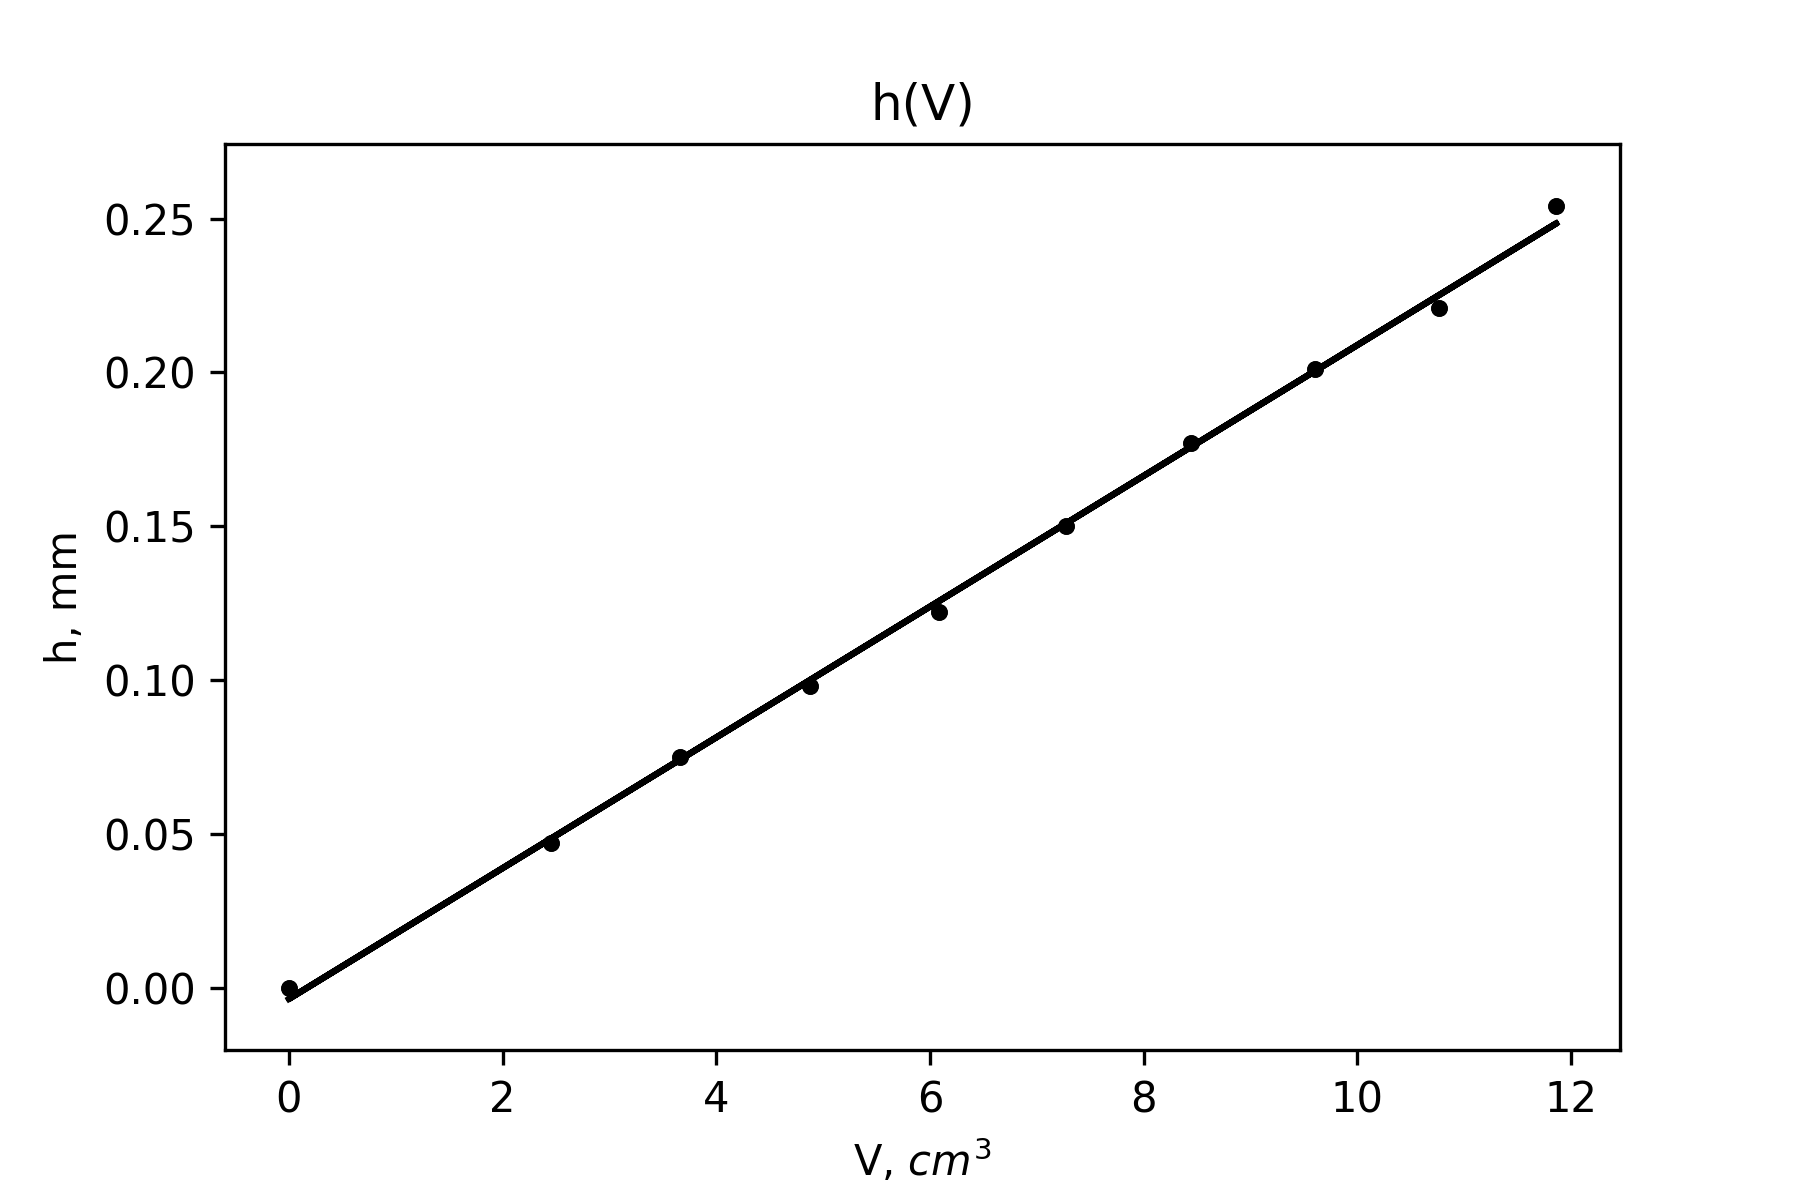
\includegraphics[width = 1  \textwidth]{plot}
\end{center}

\end{document} % конец документа